% 	INSPIRED AND MADE FROM:        
        
        %%******************************************%%
        %%                                          %%
        %%        Modello di tesi di laurea         %%
        %%            di Andrea Giraldin            %%
        %%                                          %%
        %%             2 novembre 2012              %%
        %%                                          %%
        %%******************************************%%


% I seguenti commenti speciali impostano:
% 1. 
% 2. PDFLaTeX come motore di composizione;
% 3. project-report.tex come documento principale;
% 4. il controllo ortografico italiano per l'editor.

% !TEX encoding = UTF-8
% !TEX TS-program = pdflatex
% !TEX root = project-report.tex
% !TEX spellcheck = it-IT

% PDF/A filecontents
\RequirePackage{filecontents}
\begin{filecontents*}{\jobname.xmpdata}
  \Title{Applied cryptography Cloud-Storage project report}
  \Author{Daniele Giachetto}
  \Language{eng-ENG}
  \Subject{This document describes project specifications, design choices and format of all the exchanged messages, using sequence diagrams of every used communication protocol.}
  \Keywords{Applied cryptography\sep Openssl\sep Pisa}
\end{filecontents*}

\documentclass[10pt,                    % corpo del font principale
               a4paper,                 % carta A4
               twoside,                 % impagina per fronte-retro
               openright,               % inizio capitoli a destra
               english,                 
               ]{book}    

%**************************************************************
% Importazione package
%************************************************************** 

\PassOptionsToPackage{dvipsnames}{xcolor} % colori PDF/A

\usepackage{colorprofiles}

\usepackage[a-2b,mathxmp]{pdfx}[2018/12/22]
                                        % configurazione PDF/A
                                        % validare in https://www.pdf-online.com/osa/validate.aspx

%\usepackage{amsmath,amssymb,amsthm}    % matematica

\usepackage[T1]{fontenc}                % codifica dei font:
                                        % NOTA BENE! richiede una distribuzione *completa* di LaTeX

\usepackage[utf8]{inputenc}             % codifica di input; anche [latin1] va bene
                                        % NOTA BENE! va accordata con le preferenze dell'editor

%\usepackage[italian]{babel}    % per scrivere in italiano e in inglese;
                                        % l'ultima lingua (l'italiano) risulta predefinita

\usepackage{bookmark}                   % segnalibri

\usepackage{caption}                    % didascalie

\usepackage{chngpage,calc}              % centra il frontespizio

\usepackage{csquotes}                   % gestisce automaticamente i caratteri (")

\usepackage{emptypage}                  % pagine vuote senza testatina e piede di pagina

\usepackage{epigraph}			% per epigrafi

\usepackage{eurosym}                    % simbolo dell'euro

%\usepackage{indentfirst}               % rientra il primo paragrafo di ogni sezione

\usepackage{graphicx}                   % immagini

\usepackage{hyperref}                   % collegamenti ipertestuali

\usepackage[binding=5mm]{layaureo}      % margini ottimizzati per l'A4; rilegatura di 5 mm

\usepackage{listings}                   % codici

\usepackage{microtype}                  % microtipografia

\usepackage{mparhack,fixltx2e,relsize}  % finezze tipografiche

\usepackage{nameref}                    % visualizza nome dei riferimenti                                      
\usepackage[font=small]{quoting}        % citazioni

\usepackage{subfig}                     % sottofigure, sottotabelle

\usepackage[italian]{varioref}          % riferimenti completi della pagina

\usepackage{booktabs}                   % tabelle                                       
\usepackage{tabularx}                   % tabelle di larghezza prefissata                                    
\usepackage{longtable}                  % tabelle su più pagine                                        
\usepackage{ltxtable}                   % tabelle su più pagine e adattabili in larghezza

\usepackage[toc, acronym]{glossaries}   % glossario
                                        % per includerlo nel documento bisogna:
                                        % 1. compilare una prima volta project-report.tex;
                                        % 2. eseguire: makeindex -s project-report.ist -t project-report.glg -o project-report.gls project-report.glo
                                        % 3. eseguire: makeindex -s project-report.ist -t project-report.alg -o project-report.acr project-report.acn
                                        % 4. compilare due volte project-report.tex.

\usepackage[backend=biber,style=verbose-ibid,hyperref,backref]{biblatex}
                                        % eccellente pacchetto per la bibliografia; 
                                        % produce uno stile di citazione autore-anno; 
                                        % lo stile "numeric-comp" produce riferimenti numerici
                                        % per includerlo nel documento bisogna:
                                        % 1. compilare una prima volta project-report.tex;
                                        % 2. eseguire: biber project-report
                                        % 3. compilare ancora project-report.tex.

%**************************************************************
% file contenente le impostazioni del report
%**************************************************************

%**************************************************************
% Frontespizio
%**************************************************************

% Autore
\newcommand{\myName}{Daniele Giachetto}                                    
\newcommand{\myTitle}{Applied cryptography Cloud-Storage}

% Tipo di progetto                   
\newcommand{\myDegree}{Project report}

% Università             
\newcommand{\myUni}{Università degli studi di Pisa}

% Facoltà       
\newcommand{\myFaculty}{M.Sc. Cybersecurity}

% Dipartimento
\newcommand{\myDepartment}{Department of Information Engineering}

% Titolo del docente
\newcommand{\profTitle}{Prof.}

% Docente
\newcommand{\myProf}{Michele La Manna}

% Luogo
\newcommand{\myLocation}{Pisa}

% Anno accademico
\newcommand{\myAA}{2021-2022}

% Data consegna
\newcommand{\myTime}{June 2022}


%**************************************************************
% Impostazioni di impaginazione
% see: http://wwwcdf.pd.infn.it/AppuntiLinux/a2547.htm
%**************************************************************

\setlength{\parindent}{14pt}   % larghezza rientro della prima riga
\setlength{\parskip}{0pt}   % distanza tra i paragrafi


%**************************************************************
% Impostazioni di biblatex
%**************************************************************
\bibliography{bibliografia} % database di biblatex 

\defbibheading{bibliography} {
    \cleardoublepage
    \phantomsection 
    \addcontentsline{toc}{chapter}{\bibname}
    \chapter*{\bibname\markboth{\bibname}{\bibname}}
}

\setlength\bibitemsep{1.5\itemsep} % spazio tra entry

\DeclareBibliographyCategory{opere}
\DeclareBibliographyCategory{web}

\addtocategory{opere}{womak:lean-thinking}
\addtocategory{web}{site:agile-manifesto}

\defbibheading{opere}{\section*{Riferimenti bibliografici}}
\defbibheading{web}{\section*{Siti Web consultati}}


%**************************************************************
% Impostazioni di caption
%**************************************************************
\captionsetup{
    tableposition=top,
    figureposition=bottom,
    font=small,
    format=hang,
    labelfont=bf
}

%**************************************************************
% Impostazioni di glossaries
%**************************************************************
%**************************************************************
% Glossario
%**************************************************************
\renewcommand{\glossaryname}{Glossario}

\newglossaryentry{Tor}
{
    name=\glslink{Tor}{TOR},
    text=Tor,
    sort=tor,
    description={The Onion Router è un software libero, rilasciato su licenza BSD, con un'interfaccia di gestione disponibile (Vidalia), che permette una comunicazione anonima per Internet basata sulla seconda generazione del protocollo di rete di onion routing: tramite il suo utilizzo è molto più difficile tracciare l'attività Internet dell'utente essendo finalizzato a proteggere la privacy degli utenti, la loro libertà e la possibilità di condurre delle comunicazioni confidenziali senza che vengano monitorate o intercettate.}
}


 % database di termini
\makeglossaries


%**************************************************************
% Impostazioni di graphicx
%**************************************************************
\graphicspath{{immagini/}} % cartella dove sono riposte le immagini


%**************************************************************
% Impostazioni di hyperref
%**************************************************************
\hypersetup{
    %hyperfootnotes=false,
    %pdfpagelabels,
    %draft,	% = elimina tutti i link (utile per stampe in bianco e nero)
    colorlinks=true,
    linktocpage=true,
    pdfstartpage=1,
    pdfstartview=,
    % decommenta la riga seguente per avere link in nero (per esempio per la stampa in bianco e nero)
    %colorlinks=false, linktocpage=false, pdfborder={0 0 0}, pdfstartpage=1, pdfstartview=FitV,
    breaklinks=true,
    pdfpagemode=UseNone,
    pageanchor=true,
    pdfpagemode=UseOutlines,
    plainpages=false,
    bookmarksnumbered,
    bookmarksopen=true,
    bookmarksopenlevel=1,
    hypertexnames=true,
    pdfhighlight=/O,
    %nesting=true,
    %frenchlinks,
    urlcolor=webbrown,
    linkcolor=RoyalBlue,
    citecolor=webgreen,
    %pagecolor=RoyalBlue,
    %urlcolor=Black, linkcolor=Black, citecolor=Black, %pagecolor=Black,
    pdftitle={\myTitle},
    pdfauthor={\textcopyright\ \myName, \myUni, \myFaculty},
    pdfsubject={},
    pdfkeywords={},
    pdfcreator={pdfLaTeX},
    pdfproducer={LaTeX}
}

%**************************************************************
% Impostazioni di itemize
%**************************************************************
\renewcommand{\labelitemi}{$\ast$}

%\renewcommand{\labelitemi}{$\bullet$}
%\renewcommand{\labelitemii}{$\cdot$}
%\renewcommand{\labelitemiii}{$\diamond$}
%\renewcommand{\labelitemiv}{$\ast$}


%**************************************************************
% Impostazioni di listings
%**************************************************************
\renewcommand{\lstlistingname}{Listato}
\lstset{
    language=[LaTeX]Tex,%C++,
    keywordstyle=\color{RoyalBlue}, %\bfseries,
    basicstyle=\small\ttfamily,
    language=Python,
    %identifierstyle=\color{NavyBlue},
    commentstyle=\color{Green}\ttfamily,
    stringstyle=\rmfamily,
    numbers=none, %left,%
    numberstyle=\scriptsize, %\tiny
    stepnumber=5,
    numbersep=8pt,
    showstringspaces=false,
    breaklines=true,
    frameround=ftff,
    frame=single
} 


%**************************************************************
% Impostazioni di xcolor
%**************************************************************
\definecolor{webgreen}{rgb}{0,.5,0}
\definecolor{webbrown}{rgb}{.6,0,0}


%**************************************************************
% Altro
%**************************************************************

\newcommand{\omissis}{[\dots\negthinspace]} % produce [...]

% eccezioni all'algoritmo di sillabazione
\hyphenation
{
    ma-cro-istru-zio-ne
    gi-ral-din
}

%\newcommand{\sectionname}{sezione}
%\addto\captionsitalian{\renewcommand{\figurename}{Figura}
                    %   \renewcommand{\tablename}{Tabella}}

\newcommand{\glsfirstoccur}{\ap{{[g]}}}

\newcommand{\intro}[1]{\emph{\textsf{#1}}}

%**************************************************************
% Environment per ``rischi''
%**************************************************************
\newcounter{riskcounter}                % define a counter
\setcounter{riskcounter}{0}             % set the counter to some initial value

%%%% Parameters
% #1: Title
\newenvironment{risk}[1]{
    \refstepcounter{riskcounter}        % increment counter
    \par \noindent                      % start new paragraph
    \textbf{\arabic{riskcounter}. #1}   % display the title before the 
                                        % content of the environment is displayed 
}{
    \par\medskip
}

\newcommand{\riskname}{Rischio}

\newcommand{\riskdescription}[1]{\textbf{\\Descrizione:} #1.}

\newcommand{\risksolution}[1]{\textbf{\\Soluzione:} #1.}

%**************************************************************
% Environment per ``use case''
%**************************************************************
\newcounter{usecasecounter}             % define a counter
\setcounter{usecasecounter}{0}          % set the counter to some initial value

%%%% Parameters
% #1: ID
% #2: Nome
\newenvironment{usecase}[2]{
    \renewcommand{\theusecasecounter}{\usecasename #1}  % this is where the display of 
                                                        % the counter is overwritten/modified
    \refstepcounter{usecasecounter}             % increment counter
    \vspace{10pt}
    \par \noindent                              % start new paragraph
    {\large \textbf{\usecasename #1: #2}}       % display the title before the 
                                                % content of the environment is displayed 
    \medskip
}{
    \medskip
}

\newcommand{\usecasename}{UC}

\newcommand{\usecaseactors}[1]{\textbf{\\Attori Principali:} #1. \vspace{4pt}}
\newcommand{\usecasepre}[1]{\textbf{\\Precondizioni:} #1. \vspace{4pt}}
\newcommand{\usecasedesc}[1]{\textbf{\\Descrizione:} #1. \vspace{4pt}}
\newcommand{\usecasepost}[1]{\textbf{\\Postcondizioni:} #1. \vspace{4pt}}
\newcommand{\usecasealt}[1]{\textbf{\\Scenario Alternativo:} #1. \vspace{4pt}}

%**************************************************************
% Environment per ``namespace description''
%**************************************************************

\newenvironment{namespacedesc}{
    \vspace{10pt}
    \par \noindent                              % start new paragraph
    \begin{description} 
}{
    \end{description}
    \medskip
}

\newcommand{\classdesc}[2]{\item[\textbf{#1:}] #2}
                     % file con le impostazioni personali

\begin{document}
%**************************************************************
% Materiale iniziale
%**************************************************************
\frontmatter
% !TEX encoding = UTF-8
% !TEX TS-program = pdflatex
% !TEX root = ../tesi.tex

%**************************************************************
% Frontespizio 
%**************************************************************
\begin{titlepage}

\begin{center}

\begin{LARGE}
\textbf{\myUni}\\
\end{LARGE}

\vspace{10pt}

\begin{Large}
\textsc{\myDepartment}\\
\end{Large}

\vspace{10pt}

\begin{large}
\textsc{\myFaculty}\\
\end{large}

\vspace{25pt}
\begin{figure}[htbp]
\begin{center}

\includegraphics[height=6cm]{logo-unipi}
\end{center}
\end{figure}
\vspace{30pt} 

\begin{LARGE}
\begin{center}
\textbf{\myTitle}\\
\end{center}
\end{LARGE}

\vspace{10pt} 

\begin{large}
\textsl{\myDegree}\\
\end{large}

\vspace{35pt} 

\begin{large}
\begin{flushleft}
% \textit{Relatore}\\ 
\vspace{5pt} 
\profTitle{} \myProf{} \\
\vspace{5pt}
% \textit{Correlatore}\\
\vspace{5pt}
Prof. Mariano Basile
\end{flushleft}

\vspace{0pt} 

\begin{flushright}
\textit{Student}\\ 
\vspace{5pt} 
\myName
\end{flushright}
\end{large}

\vspace{15pt}

\line(1, 0){338} \\
\begin{normalsize}
\textsc{Academic year \myAA}
\end{normalsize}

\end{center}
\end{titlepage} 
% % !TEX encoding = UTF-8
% !TEX TS-program = pdflatex
% !TEX root = ../tesi.tex

%**************************************************************
% Abstract
%**************************************************************
\cleardoublepage
\phantomsection
\pdfbookmark{Abstract}{Abstract}
\begingroup
\let\clearpage\relax
\let\cleardoublepage\relax
\let\cleardoublepage\relax

\chapter*{Abstract}

padding

%\vfill
%
%\selectlanguage{english}
%\pdfbookmark{Abstract}{Abstract}
%\chapter*{Abstract}
%
%\selectlanguage{italian}

\endgroup			

\vfill


% !TEX encoding = UTF-8
% !TEX TS-program = pdflatex
% !TEX root = ../tesi.tex

%**************************************************************
% Indici
%**************************************************************
\cleardoublepage
\pdfbookmark{\contentsname}{tableofcontents}
\setcounter{tocdepth}{2}
\tableofcontents
%\markboth{\contentsname}{\contentsname} 
\clearpage

\begingroup 
    \let\clearpage\relax
    \let\cleardoublepage\relax
    \let\cleardoublepage\relax
    %*******************************************************
    % Elenco delle figure
    %*******************************************************    
    \phantomsection
    \pdfbookmark{\listfigurename}{lof}
    \listoffigures

    \vspace*{8ex}

    %*******************************************************
    % Elenco delle tabelle
    %*******************************************************
    \phantomsection
    \pdfbookmark{\listtablename}{lot}
    \listoftables
        
    \vspace*{8ex}
\endgroup

\cleardoublepage

\cleardoublepage

%**************************************************************
% Materiale principale
%**************************************************************
\mainmatter
% !TEX encoding = UTF-8
% !TEX TS-program = pdflatex
% !TEX root = ../tesi.tex

%**************************************************************
\chapter{Introduction}
\label{cap:introduction}
%**************************************************************

%**************************************************************
\section{Project goal}

The students must implement a Client-Server application that resembles a Cloud Storage. Each user has a  ``dedicated storage'' on the server, and User A cannot access User B ``dedicated storage''. Users can Upload, Download, Rename, or Delete data to/from the Cloud Storage in a safe manner.
\begin{itemize}
	\item \textbf{Upload}: the user will upload a file found on the client machine to the server. The uploaded file size can be up to 4GB. The file will be saved with its original name, if this is not possible the file will not be uploaded;
	\item \textbf{Download}: the user will download a file from the server to the client machine. The file will be saved with its original name, if this is not possible the file will not be downloaded; 
	\item \textbf{Delete}: the user specifies a file on his ``dedicated storage'', the user will also be prompted with a choice to confirm the delete operation. The server deletes the file if it was found; 
	\item \textbf{List}: the user asks to the server the list of the filenames that are available on his ``dedicated storage''. The client shows the result to screen;
	\item \textbf{Rename}: the user specifies two filenames, the first one of the file that should be renamed and the second one the new filename desired. If the renaming operation is not possible, the filename is not changed;
\end{itemize}

Once connected to the service, the client can grafecully close the connection with the server.

%**************************************************************
\section{Assumptions \& Requisites}
Users and server will work under some assumptions that will be described in detail here: \newline{}
\textbf{Users}: 
\begin{itemize}
	\item they are pre-registered on the server;
	\item they have already the CA certificate;
	\item they have each a long-term RSA key-pair;
	\item the long-term private key is password-protected.
\end{itemize}
\textbf{Server}:
\begin{itemize}
	\item it has its own certificate signed by the CA;
	\item it knows the username of every registered user;
	\item it knows the RSA public key of every user;
	\item ``dedicated storage'' is already allocated.
\end{itemize}
When the client application starts, Server and Client must authenticate: \newline{}
\begin{itemize}
	\item server must authenticate with the public key certified by the certification authority;
	\item client must authenticate with the public key, pre-shared with the server.
\end{itemize}

During authentication a symmetric session key must be negotiated: \newline{}
\begin{itemize}
	\item the negotiation must provide Perfect Forward Secrecy;
	\item the entire session must be encrypted and authenticated;
	\item the entire session must be protected against replay attacks.
	
\end{itemize}
%**************************************************************

\section{Technology stack}

The teck stack will be listed in the Table \ref{tab:teck-stack}.
\begin{longtable}{|p{0.2\textwidth}|p{0.8\textwidth}|}
	\caption{Technology stack}
	\label{Technology stack} 
	\label{tab:teck-stack} \\
	\hline
	\textbf{Name} & \textbf{Description} \\
	\hline
	C++ & Programming language chosen, the alternatives were C or C++ and C++ with its backward compatibility and better type safety with the new operation (in constract with malloc). The code has been writter as to allow development in C changing as few things as possible. \\
	\hline
	OpenSSL & Mandatory library used to secure, authenticate and guarantee integrity of the communications. \\
	\hline
	VS code & Free text editor used to write the C++ code. \\
	\hline
	Valgrind & Programming tool for memory debugging, memory leak detection and profiling. Used mainly to debug code and find memory leak. \\
	\hline
\end{longtable}%
	

             % Introduction
% !TEX encoding = UTF-8
% !TEX TS-program = pdflatex
% !TEX root = ../tesi.tex

%**************************************************************
\chapter{Handshake \& Session key}
\label{cap:handshake-session-key}
%**************************************************************

%**************************************************************
\section{How the handshake is structured}

The handshake protocol is used to exchange a session key to encrypt and authenticate all the messages after the handshake. It guarantees perfect forward secrecy and uses nonces of 128 bits both client and server side to deny possible replay attacks. The handshake is made of 3 steps that are summarized in the following figure: \ref{fig:handshake}.

\begin{figure}[!h] 
    \centering 
    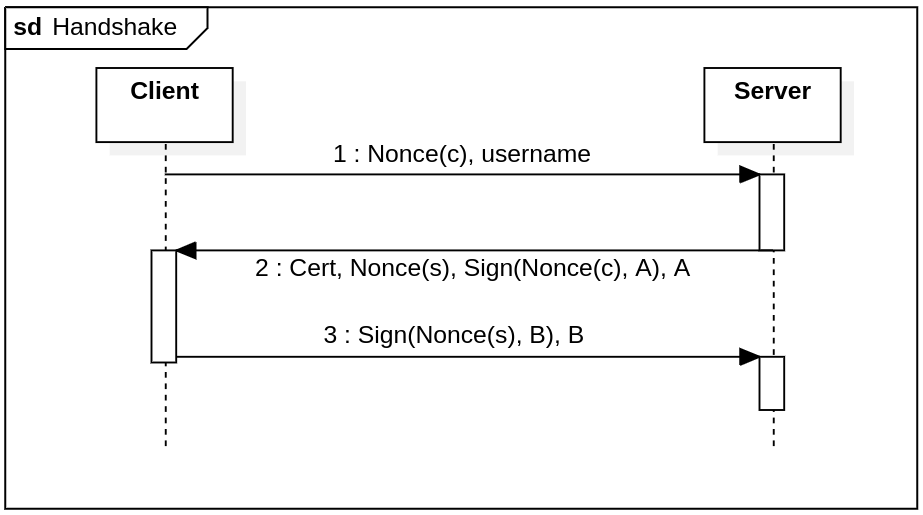
\includegraphics[width=1\columnwidth]{chapter-2/handshake.png} 
    \caption{Handshake.}
    \label{fig:handshake}
\end{figure}
\newpage{}
\begin{enumerate}
	\item client sends a random number also called nonce and the chosen username;
	\item server checks validity of username and prepares the preliminary steps to generate a shared session key:
	\begin{itemize}
		\item checks if the username does not contain invalid characters, only alphanumeric and dot characters (.) strictly not in the first position are allowed. If the username is not valid connection is closed allerting the client;
		\item checks if the username is registered, if not then the connection gets closed by sending an error message to the client;
		\item choses a random number \(\alpha\) and uses it to calculate the public Diffie-Hellman key that we will call ``A'' as A = \(g^\alpha mod p \);
		\item the server now sends his certificate, a random number and ``A''. It also signs, using SHA256 with the server private RSA key, the random number received from the client Nonce(c) and A together and sends the signature to the client.
	\end{itemize}
	\item the client checks validity of certificate and signature and generates the shared session key:
	\begin{itemize}
		\item validates server certificate using the CA;
		\item uses server public key to validate the signature received;
		\item choses a random number \(\beta\) and uses it to calculate the public Diffie-Hellman key that we will call ``B'' as B = \(g^\beta mod p \);
		\item generates shared secret Kab = \(g^{\alpha*B} mod p\);
		\item generates shared key hashing Kab with SHA256 and truncating the result to 128 bits;
		\item signs, using SHA256 with the client private RSA key, the random received Nonce(s) and ``B'';
		\item eliminates ``A'', ``B'', \(\alpha\);
		\item sends the generated signature. 
	\end{itemize}
	\item the server checks validity of signature and generates the shared session key:
	\begin{itemize}
		\item uses client public key to validate the signature received;
		\item generates shared secret Kab = \(g^{\beta*A} mod p\);
		\item generates shared key hashing Kab with SHA256 and truncating the result to 128 bits;
		\item eliminates ``A'', ``B'', \(\beta\);
	\end{itemize}	 
\end{enumerate}

%**************************************************************
\newpage{}
\section{Session key}

\subsection{How is the session key used}

The session key is used to encrypt packets using Authenticated Encryption With Associated Data (AEAD) with AES-GCM. This uses the generated symmetric key and provides authentication and integrity. This approach has been chosen based on the ease of implementation, the fact that it is less error prone and also faster. 

\begin{figure}[!h] 
    \centering 
    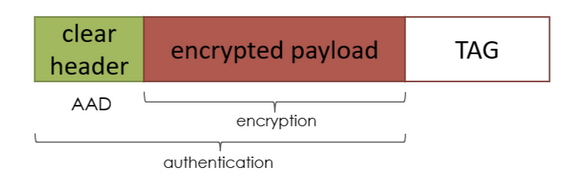
\includegraphics[width=1\columnwidth]{chapter-2/authenticated_encryption.png} 
    \caption{Authenticated Encryption message representation. In green authenticated field, in red authenticated and encrypted fields.}
    \label{fig:authenticated_encryption}
\end{figure}

\subsection{Key length}

As for key length it has been decided that the private key will be 3072 bits (384 bytes) long, while the symmetric key will be 128 bits. This decision aims at strengthening long term security with the long private key, and on the session key aims at the best tradeoff between security and overhead performance cost. 128 bits keys with the AES algorithm are the recommended length, have been deeply scrutinized and the only possible vulnerability comes with quantum computer attacks. With Grover's algorithm, a brute-force attack on a 128 bit key will result in roughly \(2^{64}\) operations to break it, which is doable but would require many resources and it won’t be possible in the near future.

%**************************************************************             % Handshake
% !TEX encoding = UTF-8
% !TEX TS-program = pdflatex
% !TEX root = ../tesi.tex

%**************************************************************
\chapter{Messages}
\label{cap:messages}
%**************************************************************

%**************************************************************
\section{Structure of packets}

There is one generic packet that will be exchanged during the client - server communication. We shall call it ``OperationPacket'' and it is made of: \newline{}
\begin{itemize}
	\item AAD (24 bytes)
	\item IV (12 bytes)
	\item PAYLOAD (variable size defined inside the AAD)
	\item TAG (16 bytes)
\end{itemize}
The AAD content is represented in the Table \ref{tab:AAD-content}.
\begin{longtable}{|p{0.4\textwidth}|p{0.2\textwidth}|}
	\caption{AAD content}
	\label{AAD content} 
	\label{tab:AAD-content} \\
	\hline
	\textbf{Content} & \textbf{Size} \\
	\hline
	Operation ID & 4 bytes \\
	\hline
	Message counter & 8 bytes \\
	\hline
	Payload length & 8 bytes \\
	\hline
	Number of Packets & 4 bytes \\
	\hline
\end{longtable}%

An in depth description of every single content of the AAD is necessary:

\begin{itemize}
	\item \textbf{Operation ID}: represents an integer number that will indicate the type of the operation to be done. The values that Operation ID can have will be listed at \ref{tab:operation-ids-list};
	\item \textbf{Message counter}: counter of the number of messages exchanged between server and client, it is used to avoid replay attack and as such must be in sync both client side and server side;
	\item \textbf{Payload length}: the payload length will be variable and this data will be used to know how many bytes to expect as payload;
	\item \textbf{Number of packets}: Some operations will send data in multiple packets, this value is used to know how many packets to expect.
\end{itemize}

\begin{longtable}{|p{0.06\textwidth}|p{0.15\textwidth}|p{0.79\textwidth}|}
	\caption{Operation ID values and description}
	\label{Operation ID list} 
	\label{tab:operation-ids-list} \\
	\hline
	\textbf{Value} & \textbf{Operation} & \textbf{Description} \\
	\hline
	 0 & ACK & Message received, the operation is allowed and can continue \\
	\hline
	 1 & UPLOAD & Client operation used to ask the server for permission to upload a local file to remote \\
	\hline
	 2 & DOWNLOAD & Client operation used to ask the server for permission to download a remote file to local \\
	\hline
	 3 & DELETE & Client operation used to ask the server for permission to delete a remote file \\
	\hline
	 4 & LIST & Client operation used to ask the server the list of remote files  \\
	\hline
	 5 & RENAME & Client operation used to ask the server to rename a remote file \\
	\hline
	 6 & LOGOUT & Client operation used to gracefully close the connection \\
	\hline
	 7 & DONE & Used to communicate that the previous operation has been completed successfully \\
	\hline
	 8 & ABORT & Message received, the operation is not allowed and cannot continue \\
	\hline
	 9 & DATA & The packet contains file data \\
	\hline
\end{longtable}%

\section{Operations} \label{sec:operations}

In this section every operation and its sequence diagram will be discussed and explained.

\subsection{Upload}
\begin{enumerate} 
	\item client, after validating filename, file existance and size, sends OperationPacket with payload made of the filename and AAD made of message counter and: \newline{}
	\begin{itemize}
		\item operation ID = UPLOAD;
		\item number of packets that will be sent to server;
		\item payload length: the size of the filename.
	\end{itemize}
	\item server validates the request checking the filename and if the file does not exists already and sends ACK if valid, otherwise ABORT;
	\item client starts sending in order but asynchronously data packets containing the content of the files;
	\item server reads and validates every packets, checking if they are being received in the correct order. When the server finishes reading all the packets it sends a DONE.

\end{enumerate}

\begin{figure}[!h] 
    \centering 
    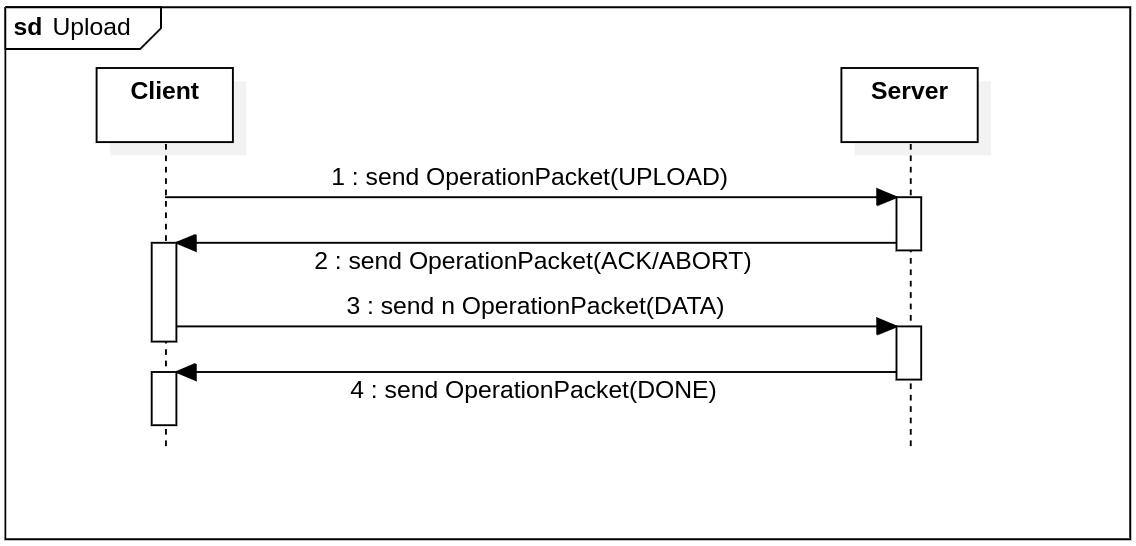
\includegraphics[width=1\columnwidth]{chapter-3/Upload.png} 
    \caption{Upload operation.}
    \label{fig:upload_operation}
\end{figure}

\newpage{}

\subsection{Download}
\begin{enumerate}
	\item client, after validating filename and file existance, sends OperationPacket with payload made of the filename and AAD made of message counter and: \newline{}
	\begin{itemize}
		\item operation ID = DOWNLOAD;
		\item payload length: the size of the filename.
	\end{itemize}
	\item server validates the request checking filename and if the file exists and sends ACK if valid, otherwise ABORT;
	\item client sends ACK;
	\item server starts sending in order but asynchronously data packets containing the content of the files;
	\item client reads and validates every packets, checking if they are being received in the correct order. When the client finishes reading all the packets it sends a DONE.
\end{enumerate}

\begin{figure}[!h] 
    \centering 
    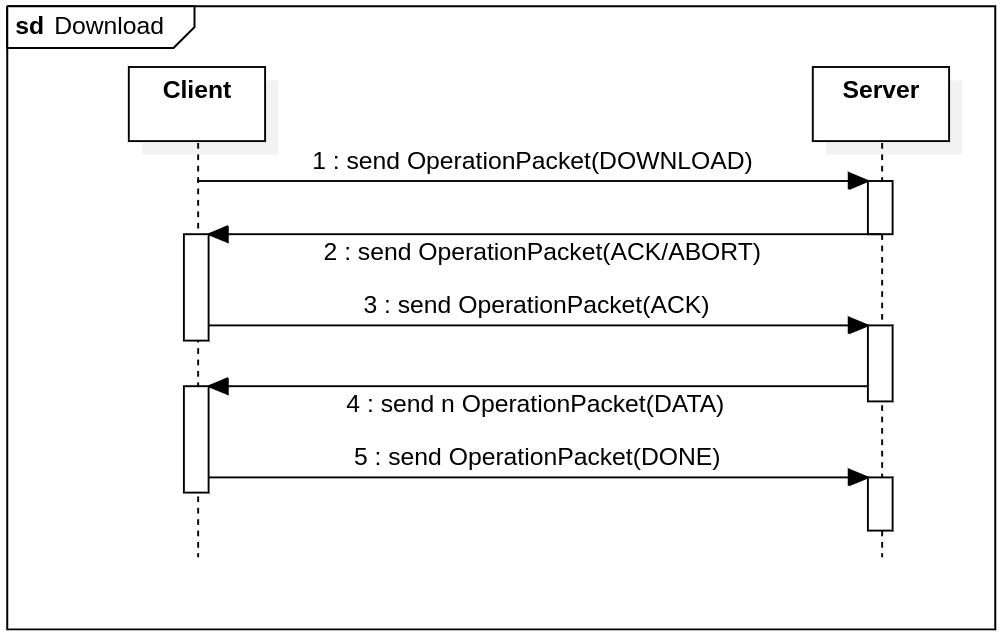
\includegraphics[width=1\columnwidth]{chapter-3/Download.png} 
    \caption{Download operation.}
    \label{fig:download_operation}
\end{figure}
\newpage{}
\subsection{List}
\begin{enumerate}
	\item client sends OperationPacket LIST;
	\item server sends OperationPacket DATA containing all the filenames found and validated by the server on the remote folder, separated by ','. Ex: file1,file2,file3 ;
	\item client reads the OperationPacket and splits the received payload in strings, validates them and display them to console.
	
\end{enumerate}
\begin{figure}[!h] 
    \centering 
    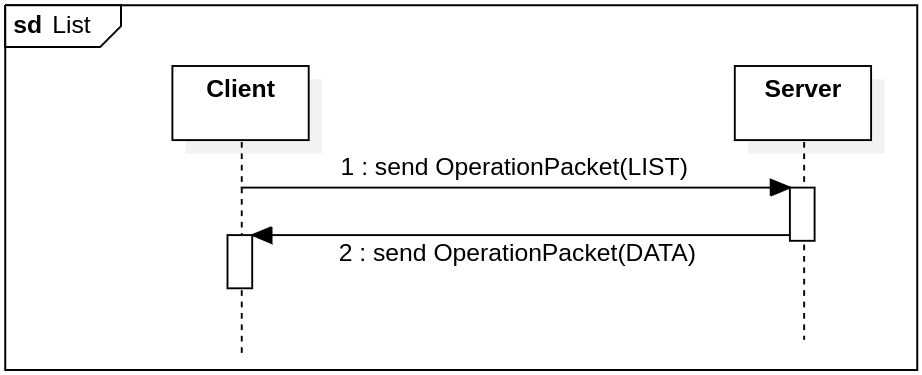
\includegraphics[width=1\columnwidth]{chapter-3/List.png} 
    \caption{List operation.}
    \label{fig:list_operation}
\end{figure}

\subsection{Delete}
\begin{enumerate}
	\item client inputs a filename, validates the input and if valid checks for client confirmation of this destructive operation. The check is made client side because, if someone modified the client source code, then it would be as trivial to skip the client side check as it would to send an automatic ACK message after the server asks for confirmation. This means that a server side check will not provide benefit nor in security nor in speed while putting the check client side the security will be the same but sending useless packets will be avoided;
	\item client sends OperationPacket DELETE with payload containing filename;
	\item server validates the request checking filename and if the file exists and delete file and sends DONE if valid, otherwise ABORT;
\end{enumerate}

\begin{figure}[!h] 
    \centering 
    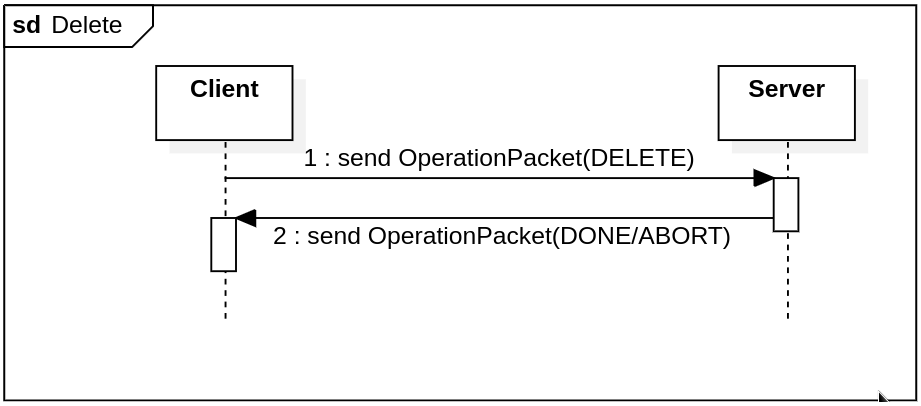
\includegraphics[width=1\columnwidth]{chapter-3/Delete.png} 
    \caption{Delete operation.}
    \label{fig:delete_operation}
\end{figure}

\subsection{Rename}
\begin{enumerate}
	\item client first inputs the file to rename and after that the name that he wants to rename it to. Every step of the input is validated;
	\item client sends OperationPacket RENAME containing the two filenames as payload, separated by ','. Ex: fileold.example,filenew.txt ;
	\item server reads the OperationPacket and splits the received payload in two strings, old and new name. It validates the two, checks if the old filename exists in the remote folder and then renames it to the desired new name. If this was successful sends DONE, otherwise ABORT.
\end{enumerate}

\begin{figure}[!h] 
    \centering 
    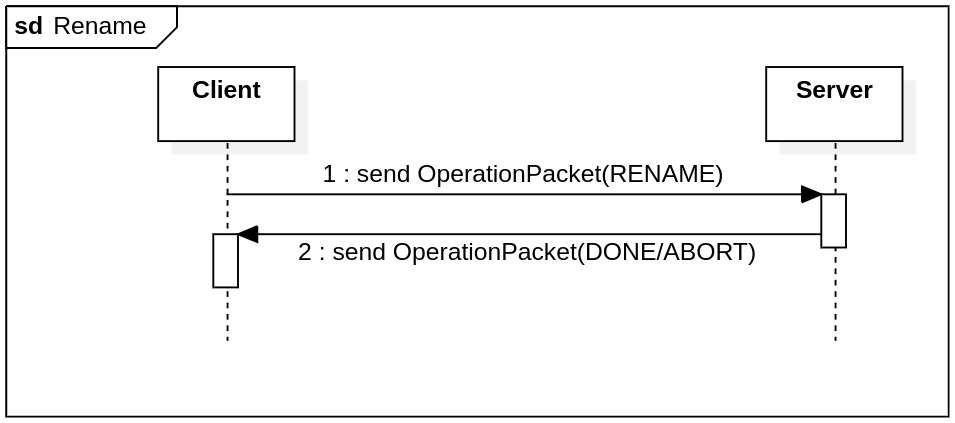
\includegraphics[width=1\columnwidth]{chapter-3/Rename.png} 
    \caption{Rename operation.}
    \label{fig:rename_operation}
\end{figure}
\newpage{}
\subsection{Logout}
\begin{enumerate}
	\item client sends OperationPacket LOGOUT;
	\item server answers with OperationPacket ACK;
	\item client asks the user to confirm the operation;
	\item if the operation was confirmed sends DONE to server and closes the connection, otherwise ABORT;
	\item server reads the OperationPacket and if DONE it closes the connection on its part, otherwise it ignores the previous request and keeps the connection going.
\end{enumerate}


\begin{figure}[!h] 
    \centering 
    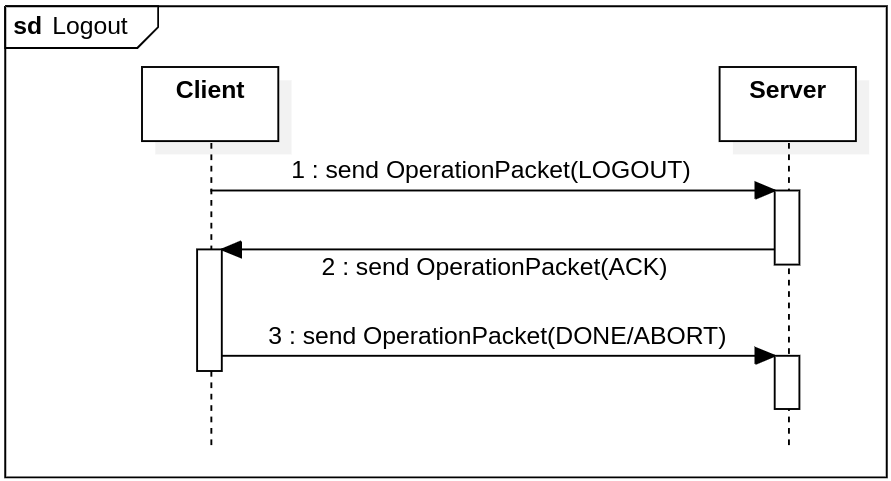
\includegraphics[width=1\columnwidth]{chapter-3/Logout.png} 
    \caption{Logout operation.}
    \label{fig:logout_operation}
\end{figure}
             % Messages
%\input{capitoli/capitolo-4}             % Progettazione e sviluppo
%\input{capitoli/capitolo-5}             % Verifica e validazione
%\input{capitoli/capitolo-6}             % Conclusioni
\appendix                               
%\input{capitoli/capitolo-A}             % Appendice A

%**************************************************************
% Materiale finale
%**************************************************************
%\backmatter
%\printglossary[title={Glossario}]
% % !TEX encoding = UTF-8
% !TEX TS-program = pdflatex
% !TEX root = ../tesi.tex

%**************************************************************
% Bibliografia
%**************************************************************

\cleardoublepage
\chapter{Bibliografia}

\nocite{*}
% Stampa i riferimenti bibliografici
\printbibliography[heading=subbibliography,title={Riferimenti bibliografici},type=book]

% Stampa i siti web consultati
\printbibliography[heading=subbibliography,title={Siti web consultati},type=online]


\end{document}
